%%%%%%%%%%%%%%%%%%%%%%%%%%%%%%%%%%%%%%%%%
% String Theory Labs OSC Namespace Template
%
% Note:
% If you are using Apple OS X, go into structure.tex and uncomment the font
% specifications for OS X and comment out the default specifications - this will
% drastically increase how good the document looks. You will now need to
% compile with XeLaTeX.
%
%%%%%%%%%%%%%%%%%%%%%%%%%%%%%%%%%%%%%%%%%

\documentclass[usletter,12pt]{article} % The default font size is 12pt on A4 paper, change to 'usletter' for US Letter paper and adjust margins in structure.tex

\usepackage{amsmath, mathabx}
\usepackage{mathtools}
\usepackage{mathspec}
\usepackage{enumitem}

\usepackage[framed]{mcode}
\usepackage{python}
\lstset{
    frame=single,
    breaklines=true,
    postbreak=\raisebox{0ex}[0ex][0ex]{\ensuremath{\color{red}\hookrightarrow\space}}
}


%%%%%%%%%%%%%%%%%%%%%%%%%%%%%%%%%%%%%%%%%
% Contract
% Structural Definitions File
% Version 1.0 (December 8 2014)
%
% Created by:
% Vel (vel@latextemplates.com)
% 
% This file has been downloaded from:
% http://www.LaTeXTemplates.com
%
% License:
% CC BY-NC-SA 3.0 (http://creativecommons.org/licenses/by-nc-sa/3.0/)
%
%%%%%%%%%%%%%%%%%%%%%%%%%%%%%%%%%%%%%%%%%

%----------------------------------------------------------------------------------------
%	PARAGRAPH SPACING SPECIFICATIONS
%----------------------------------------------------------------------------------------

%\setlength{\parindent}{0mm} % Don't indent paragraphs
\usepackage{indentfirst}

\setlength{\parskip}{2.5mm} % Whitespace between paragraphs

%----------------------------------------------------------------------------------------
%	PAGE LAYOUT SPECIFICATIONS
%----------------------------------------------------------------------------------------

\usepackage{geometry} % Required to modify the page layout\

\usepackage[final]{pdfpages} % Allows pdf inclusion

\usepackage{float}

\usepackage{hyperref}
\hypersetup{
    colorlinks=true, %set true if you want colored links
    linktoc=all,     %set to all if you want both sections and subsections linked
    linkcolor=blue,  %choose some color if you want links to stand out
    urlcolor=cyan
}

%\renewcommand{\thesection}{\Roman{section}}

\usepackage[tocindentauto]{tocstyle}
\usetocstyle{KOMAlike} %the previous line resets it

\setlength{\textwidth}{16cm} % Width of the text on the page
\setlength{\textheight}{24.5cm} % Height of the text on the page

\setlength{\oddsidemargin}{0cm} % Width of the margin - negative to move text left, positive to move it right

% Uncomment for offset margins if the 'twoside' document class option is used
%\setlength{\evensidemargin}{-0.75cm} 
%\setlength{\oddsidemargin}{0.75cm}

\setlength{\topmargin}{-1.95cm} % Reduce the top margin

%----------------------------------------------------------------------------------------
%	FONT SPECIFICATIONS
%----------------------------------------------------------------------------------------

% If you are running Apple OS X, uncomment the next 4 lines and comment/delete the block below, you will now need to compile with XeLaTeX but your document will look much better

% \usepackage[cm-default]{fontspec}
% \usepackage{xunicode}

%\setsansfont[Mapping=tex-text,Scale=1.1]{Gill Sans}
%\setmainfont[Mapping=tex-text,Scale=1.0]{Hoefler Text}

%-------------------------------------------

%\usepackage[utf8]{inputenc} % Required for including letters with accents
%\usepackage[T1]{fontenc} % Use 8-bit encoding that has 256 glyphs

%\usepackage{avant} % Use the Avantgarde font for headings
%\usepackage{mathptmx} % Use the Adobe Times Roman as the default text font together with math symbols from the Sym­bol, Chancery and Com­puter Modern fonts

%----------------------------------------------------------------------------------------
%	SECTION TITLE SPECIFICATIONS
%----------------------------------------------------------------------------------------

\usepackage{titlesec} % Required for modifying section titles

%\titleformat{\section} % Customize the \section{} section title
%{\sffamily\large\bfseries} % Title font customizations
%{\thesection} % Section number
%{16pt} % Whitespace between the number and title
%{\large} % Title font size
%\titlespacing*{\section}{0mm}{7mm}{0mm} % Left, top and bottom spacing around the title

%\titleformat{\subsection} % Customize the \subsection{} section title
%{\sffamily\normalsize\bfseries} % Title font customizations
%{\thesubsection} % Subsection number
%{16pt} % Whitespace between the number and title
%{\normalsize} % Title font size
%\titlespacing*{\subsection}{0mm}{5mm}{0mm} % Left, top and bottom spacing around the title % Input the structure.tex file which specifies the document layout and style

%----------------------------------------------------------------------------------------
%	DYNAMIC CONTRACT INFORMATION
%----------------------------------------------------------------------------------------

% Your name and company name
\newcommand{\Authors}{Wisam Reid \& Iran Roman}
\newcommand{\CompanyName}{Toward a Dynamic Model of Parkinson's Disease}

% Your email address
\newcommand{\YourEmail}{wisam@ccrma.stanford.edu}
% The client's name
\newcommand{\SubTitle}{Thoughts \& Research Notes}	


%----------------------------------------------------------------------------------------

\begin{document}

%----------------------------------------------------------------------------------------
%	TITLE PAGE
%----------------------------------------------------------------------------------------

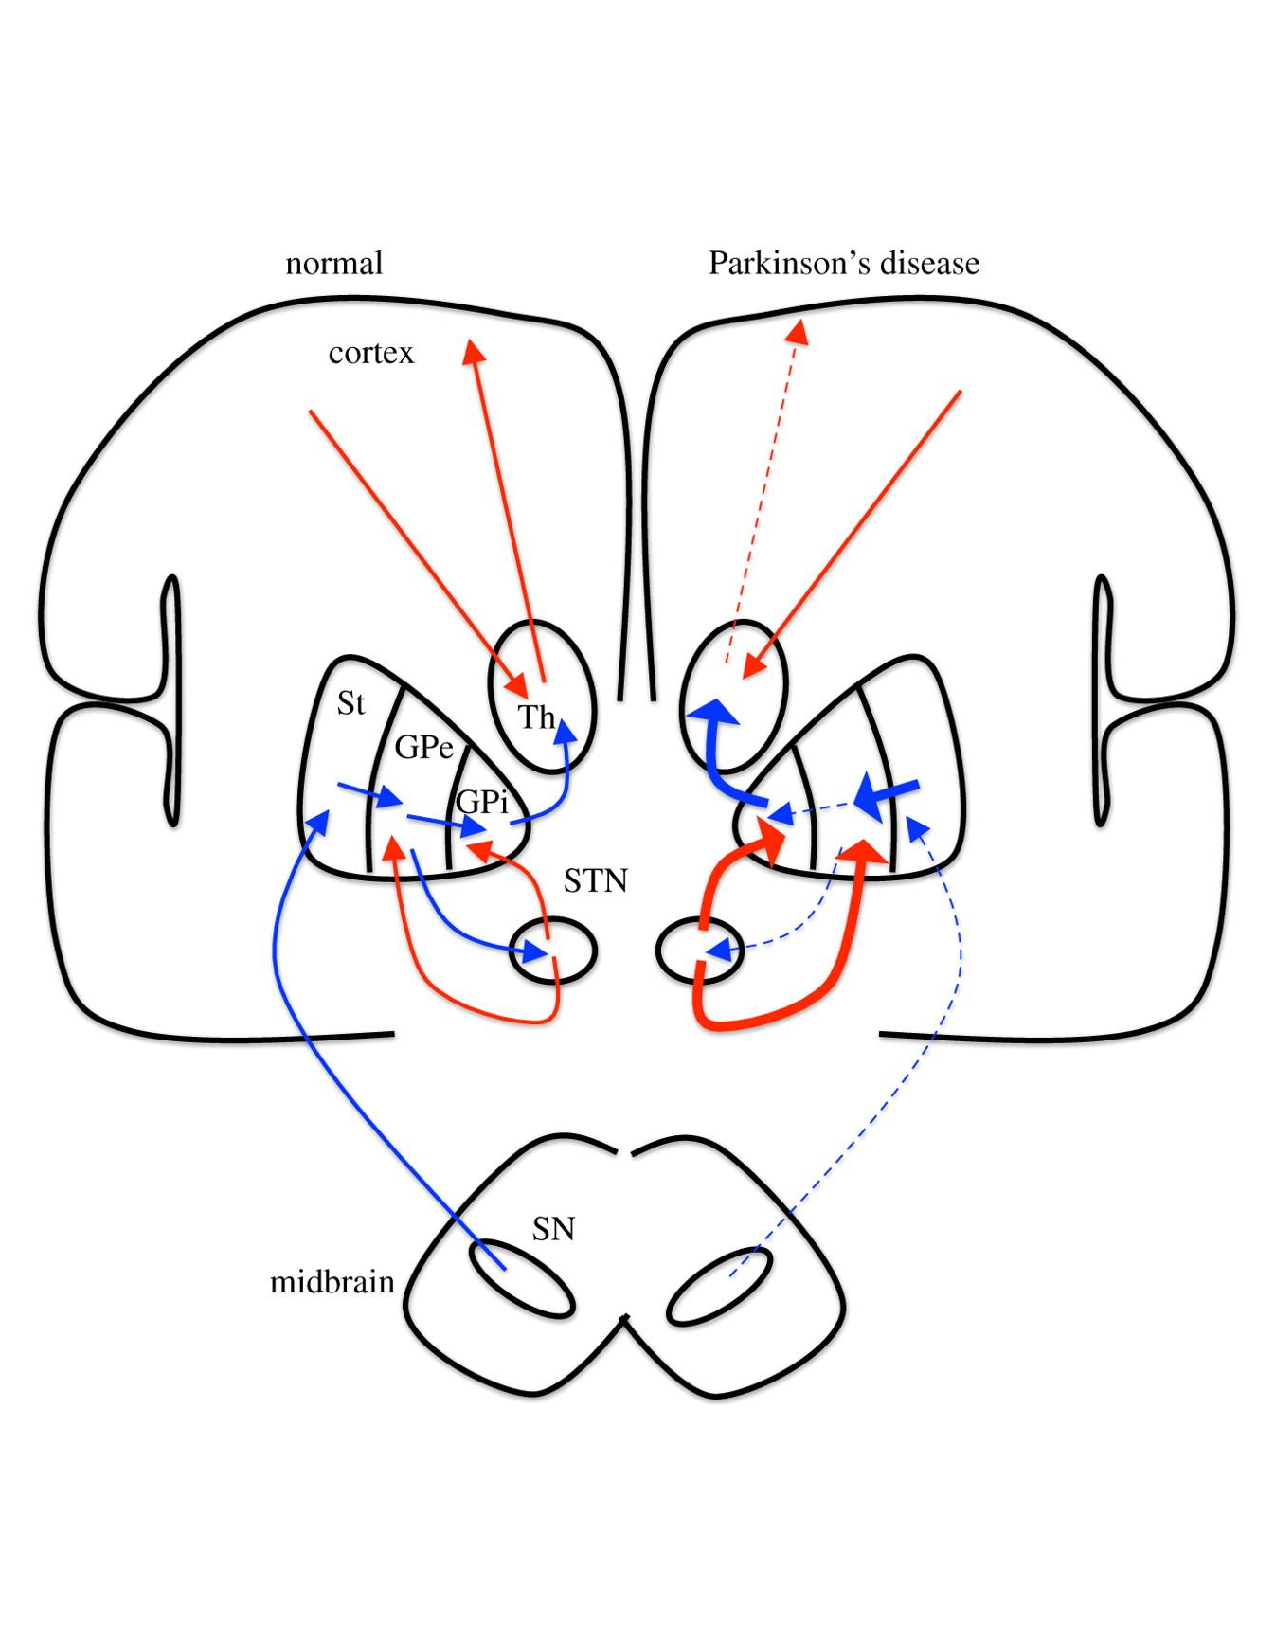
\includepdf{images/Parkinons_Diagram.pdf}

\begin{center}

\vspace*{\fill} % Add whitespace below to center the title page content

{\textbf{\Huge \CompanyName}}\\ [1.5cm]
{\LARGE \SubTitle}\\ [1.5cm]

By \Authors\\

\vspace*{\fill} % Add whitespace below to center the title page content

\end{center}

\newpage

\tableofcontents

\newpage

%----------------------------------------------------------------------------------------
%	Project Summary
%----------------------------------------------------------------------------------------

\section{A Brief Overview}\label{overview}

\noindent
We are working toward a dynamic model of Parkinson’s Disease (PD).  

\noindent
As a first step we are building a model of healthy coupled brain oscillation during movement coordination in healthy subjects and stroke victims, as observed by Takako Fujioka’s MEG studies and double-blinded randomized clinical trials on stroke recovery.  We then want to build up towards a PD model that will hold up against everything currently known about PD. 


%----------------------------------------------------------------------------------------
%	The Data
%----------------------------------------------------------------------------------------

\section{The Data}

\noindent
MEG data from healthy subjects and stroke victims during a tap based rhythm task.  Collected by Takako Fujioka. \cite{fujioka2009beta}  \cite{jamali2014neuromagnetic}


%----------------------------------------------------------------------------------------
%	A simple baseline conceptual model
%----------------------------------------------------------------------------------------

\section{A Simple Baseline Conceptual Model}

\noindent
This is an attempt at replicating studies indicating that beta ERD occurs after hearing a beat, and at that point gamma ERS occurs.  Below is a Matlab script and the plots that it generates.  

%---------------------------------------------------
%	Plots
%---------------------------------------------------
\subsection{Plots}

\begin{figure}[H]
\centering
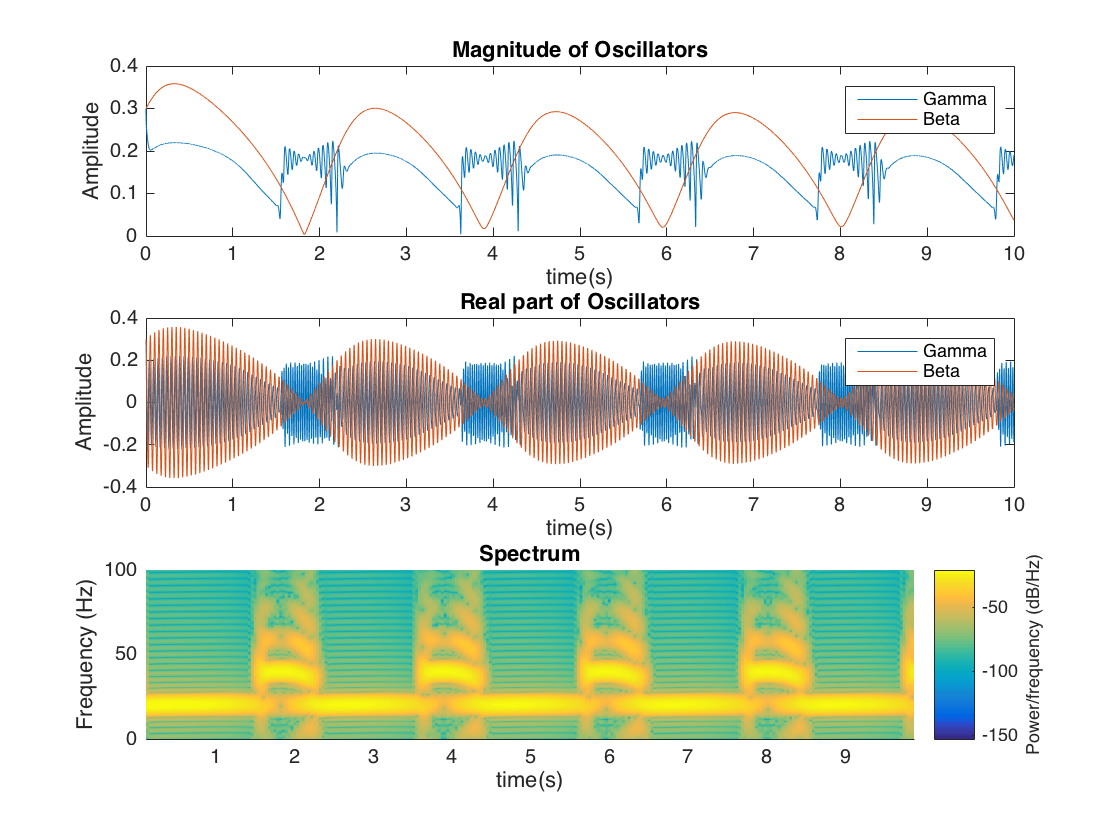
\includegraphics[scale=0.275]{images/simple_model}
\caption{A "beta" oscillator driving a "gamma" oscillator. The "beta" oscillator is modulated by a 0.5 Hz envelope, which is supposed to emulate be the result of stimulation by listening of an isochronous rhythm. The "gamma" oscillator is tuned to a limit cycle and oscillates at its frequency only when the beta oscillator has a low amplitude.}
\label{fig:simple_model}
\end{figure}

\begin{figure}[H]
\centering
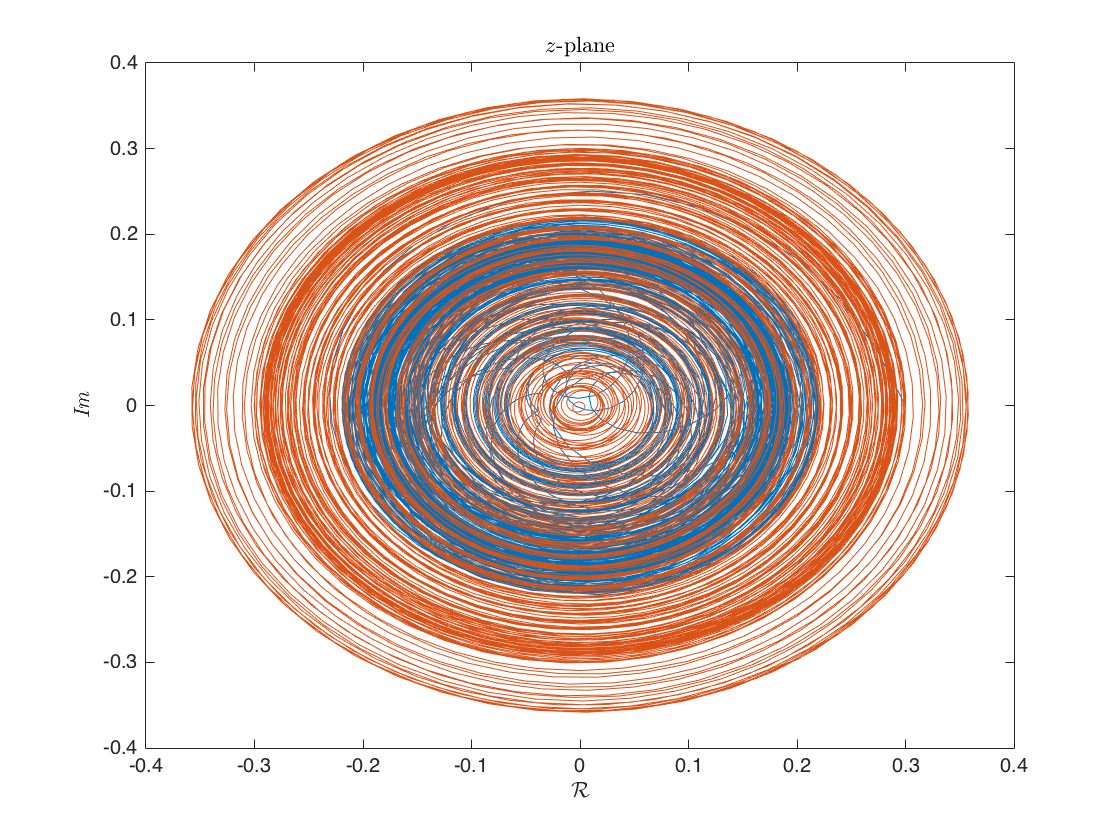
\includegraphics[scale=0.275]{images/simple_model_z}
\caption{The "beta" and "gamma" oscillators in the $z$-plane}
\label{fig:simple_model_z}
\end{figure}

%---------------------------------------------------
%	Matlab Code 
%---------------------------------------------------

\subsection{Matlab Code}

\begin{lstlisting}[language=Matlab]
%%%%%%%%%%%%%%%%%%%%%%%%%%%%%%%%%%%%%%%%%%%%
%
% Authors: Iran Roman & Wisam Reid 
%
% This script shows a limit cycle oscillator 
% in the beta band (20Hz)
%
%%%%%%%%%%%%%%%%%%%%%%%%%%%%%%%%%%%%%%%%%%%%
%% CLEAN AND CLEAR

clc;
clear;
close all;

%% Include the GrFNN toolbox
addpath(genpath('~/Documents/GrFNNToolbox/'))

%% the output of beta drives a gamma oscillator

dzdt = @(t,z,alpha,beta1,beta2,epsilon,F,omega0)  ...        
    [z(1)*(100*alpha + 1i*2*pi*40 + 200*beta1*abs(z(1))^2 + ...     
    (epsilon*beta2*abs(z(1))^4)/(1-epsilon*abs(z(1))^2)) + 3.5*(z(2)*exp(pi)); ...
    (z(2)*(alpha + 1i*2*pi*20 + beta1*abs(z(2))^2 + ... % beta layer
    (epsilon*beta2*abs(z(2))^4)/(1-epsilon*abs(z(2))^2)) + ...   
    F*exp(1i*omega0*t))]; % input to beta

%% parameters 

% for the limit cycle oscillator
z0 = 0.3;
alpha = 1;
beta1 = -15;
beta2 = -1;
epsilon = 1;
F = 0.5;
f0 = 20.5;
omega0 = 2*pi*f0;

% for time
fs = 1000;
dur = 10; % in seconds
T = 1/fs;
time = 0:T:dur;

%% integrate the ode to obtain the amplitude

[t,z] = ode45(@(t,z) dzdt(t,z,alpha,beta1,beta2,epsilon,F,omega0),time,[z0,z0]);

% extract information
r = abs(z);
dr2dt = diff(r(:,1));
dr1dt = diff(r(:,2));

%% Plot

figure(2)
plot(z)
xlabel('$\mathcal{R}$','Interpreter','latex')
title('$z$-plane','Interpreter','latex')
ylabel('$\textit{Im}$','Interpreter','latex')

figure(3)
subplot(3,1,1)
plot(time,r)
title('Magnitude of Oscillators')
ylabel('Amplitude')
xlabel('time(s)')
legend('Gamma','Beta')
subplot(3,1,2)
plot(time,real(z))
title('Real part of Oscillators')
legend('Gamma','Beta')
ylabel('Amplitude')
xlabel('time(s)')
subplot(3,1,3)
spectrogram((z(:,1)),kaiser(256,5),220,20000,fs,'yaxis')
title('Spectrum')
ylim([0 100])
xlabel('time(s)')

\end{lstlisting}


%---------------------------------------------------
% To Do 
%---------------------------------------------------
\subsection{To Do}

\noindent 
After Iran's meeting with Takako, we know that this needs some refinement.  Since, in healthy subjects gamma does not spontaneously oscillate. Beta does, and Gamma must be evoked by sound.  Beta is always oscillating and gamma gives exogenous or endogenous input to affect beta. High gamma gives rise to the desynchronization of beta \cite{jenkinson2011new}. 

\noindent 
In contrast, with the advance of PD, dopamine is depleted in the basal ganglia, and experimental evidence suggests that this depletion has an effect on the synaptic weights of the subthalamic nucleus-external globus pallidus (STN-GPe) network. This gives rise to constant beta oscillation and obstructs motor coordination.  In deep brain stimulation (DBS) patients, 20 Hz stimulation is ineffective, with 40 Hz gamma nothing happens (no beta desynchronization), and with high gamma 80 Hz there is improvement. 

\noindent 
\textbf{We plan to modify this baseline model to accommodate the correct healthy behavior.}


%---------------------------------------------------
% Proposed Methods
%---------------------------------------------------

\section{Proposed Method} \label{proposed-method}

\noindent 
We want to move toward something much more interesting.

\noindent 
Said quickly, we want to get away from “engineering” bifurcation parameters.  We want to marry ONNs that fit their parameters directly from brain data, with dynamic causal analysis. 

%---------------------------------------------------
% Some Philosophical Alignment
%---------------------------------------------------

\subsection{Some Philosophical Alignment}

\noindent 
As you already know, Iran and I are both interested in Oscillatory/Spiking Neural Networks (O/SNN) and with that comes a lot of the interesting questions. 
%that I think you have also been exploring yourself.  
We want to model the brain in the framework of Bifurcation Theory, but modeling at what scale is appropriate or most beneficial?  Without going on a tangent here, I would say that those answers depend on what you are measuring and what you are trying to model.  Here are some papers that are currently inspiring this thought process \cite{izhikevich2004model} \cite{izhikevich2008large} \cite{large2015neural}. 

%--------------------------------------------------------
%Fitting Bifurcation Parameters to Data
%--------------------------------------------------------

\subsection{Fitting Bifurcation Parameters to Data}

\noindent 
My literature review started with some published bifurcation models \cite{merrison2013interactive} \cite{nevado2011bifurcation} but this quickly lead me to a particularly interesting model implemented by Pavlides et al.  Their model fixes some of its parameters from known physiology and fits others (e.g. neuronal coupling weights) with a cost function directly from data.  The cost function constrains the solution including penalizing for losses of known functionality when simulating a variety of lesions in the Basal Ganglia \cite{pavlides2015computational} \cite{tachibana2011subthalamo}.

\noindent 
If you are interested, the Pavlides et al. paper does an amazing job of explaining how Tachibana et al. physiological work on macaques, which involved blocking pathways between brain regions implicated in PD, has invalidated several formally proposed PD models.  Their model claims to uphold appropriate behavior when simulating a variety of lesions in the Basal Ganglia. This is an important property I would like to capture in our model as well.

%--------------------------------------------------------
% Causality Analysis
%--------------------------------------------------------

\subsection{Causality Analysis}

\noindent 
I am also inspired by PD models that leverage causality analysis.  There are many recent models using Granger Causality (GC) \cite{kerr2013cortical} \cite{florin2016parkinson} or a more recent extension, Dynamic Causal Modeling (DCM) \cite{sheikhattar2016dynamic}.  I just recently ran into Karl J. Friston’s impressive body of work on DCM and I am now staring down the barrel of yet another needed deep literature review \cite{razi2016connected} \cite{zeller2016dynamic} \cite{penny2009dynamic} \cite{bajaj2016bridging}.

\noindent 
I think causality analysis needs to be incorporated into models like Pavlides et al. While understanding how neural populations are connected is powerful, DCM could help us understand the directional flow of information between neural populations.  The difference between functional and effective connectivity.

%--------------------------------------------------------
% Granger Causality Analysis
%--------------------------------------------------------

\subsubsection{Granger Causality Analysis}

\noindent 
In a nutshell... with GC, one examines how to best predict the future of a neuron: using either the entire ensemble or the entire ensemble except a certain target neuron.  The GC test is a statistical hypothesis test for determining whether one time series is useful in forecasting another, disambiguating correlations from causal relationships. 

\noindent 
As extra motivation for this analysis, MEG is especially equipped to overcome the common challenges/pitfalls of time-series causality analysis such as \cite{ding2014analyzing}: 

\begin{enumerate}
\item common reference  
\item volume conduction
\end{enumerate}

\noindent 
\textit{Note:} There is much greater detail on this in my \hyperref[extra-material]{literature review slides}.

%--------------------------------------------------------
% Dynamic Causal Modeling
%--------------------------------------------------------

\subsubsection{Dynamic Causal Modeling}

\noindent
Given that we want to model the network dynamics, DCM is a logical extension of GC that overcomes many of the shortcomings of GC in this setting.

\noindent
Added benefits of DCM:
\begin{enumerate}
\item Unlike Bayesian Networks, the graphs used in DCM can be cyclic
\item Unlike Structural Equation modelling and Granger causality, DCM does not depend on the theory of Martingales, i.e., it does not assume that random fluctuations' are serially uncorrelated.
\item DCM Bayesian predictions could overcome artifactual GC modulations induced by averaging event-related responses, and GC issues with phase coherence.
\end{enumerate}

\noindent 
In contrast to many causal models, DCM does not look for statistical dependencies among measured time-series directly. Instead, it combines a biophysical model of the hidden (latent) dynamics with a forward model that translates hidden states into predicted measurements.  

\noindent 
This provides a general framework, allowing us to plug in interchangeable models for the underlying neural activity given measured (hemodynamic or electromagnetic) responses over the sensors considered.  The hidden states cover any neurophysiological or biophysical variables needed to form the observations and bayesian inversion furnishes the marginal likelihood (evidence) of the model and the posterior distribution of its parameters (e.g., neuronal coupling strengths). 

\newpage

%---------------------------------------------------
%	Appendix
%---------------------------------------------------

\section{Appendix: Extra Material}\label{extra-material}

\noindent 
A verbose compilation of my thoughts from my literature review can be accessed \href{https://docs.google.com/presentation/d/1RW2VhdHcTehgb-biTPHkPg3PplrurAugfN0Y48rieqc/edit?usp=sharing}{here}.

%%%%%%%%%%%%%%%%%%%%%%%%%%%%%%%%%%%%%%%
%%%%%%%%%%%%%%%% REFERENCES %%%%%%%%%%%%%%%%
%%%%%%%%%%%%%%%%%%%%%%%%%%%%%%%%%%%%%%%

%\bibliographystyle{apalike}
 \bibliographystyle{unsrt}
\bibliography{ref}

\end{document}